\section{Multidisciplinary Shape Sensitivity Analysis}
% =============================
The shape sensitivity analysis for the coupled multidisciplinary problem is built on the work done in Chapter \ref{ch:shapeSenwithIB}. However, in this chapter, we are also including the shape sensitivity effects on the structural side. To do so, we differentiate Equations \eqref{eq:C5_fluidGE} and \eqref{eq:C5_solidGE} alongside the kinematic and dynamic constraints of Equation \eqref{eq:C5_FSIconstraints} with respect to shape design variable, $b$. The sensitivity equations for the fluid and solid domains are shown in Equation \eqref{eq:C5_fluidSA} and \eqref{eq:C5_solidSA}, respectively.
%
\begin{subequations}\label{eq:C5_fluidSA}
\begin{align}
	&\rho^f \frac{\partial}{\partial t} \left( \frac{\partial \mathbf{u}^f}{\partial b} \right) + 
	\rho^f \frac{\partial \mathbf{u}^f}{\partial b} \cdot \nabla \mathbf{u}^f +
	\rho^f \mathbf{u}^f \cdot \nabla \left( \frac{\partial \mathbf{u}^f}{\partial b} \right) = 
	\nabla \cdot \left( \frac{\partial \mathbf{\sigma}^f}{\partial b} \right) +
	\rho^f \frac{\partial \mathbf{f}^f}{\partial b}
	\\
	&\nabla \cdot \left( \frac{\partial \mathbf{u}^f}{\partial b} \right) = 0
	\\
	&\frac{\partial \mathbf{\sigma}^f}{\partial b} = 
	\mu \left[ \nabla \left( \frac{\partial \mathbf{u}^f}{\partial b} \right) + 
	           \nabla \left( \frac{\partial \mathbf{u}^f}{\partial b} \right)^T \right] - 
	\frac{\partial p^f}{\partial b} \mathbf{I}
\end{align}
\end{subequations}
%
\begin{subequations}\label{eq:C5_solidSA}
\begin{align}
	\rho^s \frac{\partial \dot{\mathbf{u}}^s}{\partial b} &= 
	\nabla \cdot \left( \frac{\partial \sigma^s}{\partial b} \right) + 
	\frac{\partial \mathbf{f}^s}{\partial b}
	\\
	\frac{\partial \mathbf{\epsilon^s}}{\partial b} &=
	\frac{1}{2}
	\left[ \nabla \frac{\partial \mathbf{d}^s}{\partial b} + \nabla \left( \frac{\partial \mathbf{d}^s}{\partial b} \right)^T \right]
	\\
	\frac{\partial \mathbf{\sigma}^s}{\partial b} &= 
	\frac{\partial \mathbf{C}}{\partial b} : \mathbf{\epsilon}^s + 
	\mathbf{C} : \frac{\partial \mathbf{\epsilon}^s}{\partial b}
\end{align}
\end{subequations}
%
%
\begin{subequations}\label{eq:C5_FSIconstraintsSA}
\begin{align}
	\frac{\partial \mathbf{u}^s}{\partial b} - 
	\frac{\partial \mathbf{u}^f}{\partial b} &= 0
	\\
	\frac{\partial \mathbf{\sigma}^s}{\partial b} \cdot \mathbf{n} - 
	\frac{\partial \mathbf{\sigma}^f}{\partial b} \cdot \mathbf{n} &= 0
\end{align}
\end{subequations}
%
As shown in Equations \eqref{eq:C5_fluidSA} and \eqref{eq:C5_solidSA}, to solve the sensitivity equations we need to obtain the solution of the governing equation ($\mathbf{u}^f$, $\mathbf{\epsilon^s}$). Therefore, we are proposing to use the flowchart of Figure \ref{fig:C5_SAflowchart} for the coupled multidisciplinary sensitivity analysis. The sensitivity calculation process starts by solving the Navier-Stokes equation and mapping the pressure to the structural domain to calculate the deformation in the structural domain. The solution of the Navier-Stokes and Elasticity equations are then fed to the sensitivity solver to calculate the sensitivity response. This loop is continued until a convergence for the governing equations is reached or the process is stopped manually. 
%
\begin{figure}[H]
    \centering
    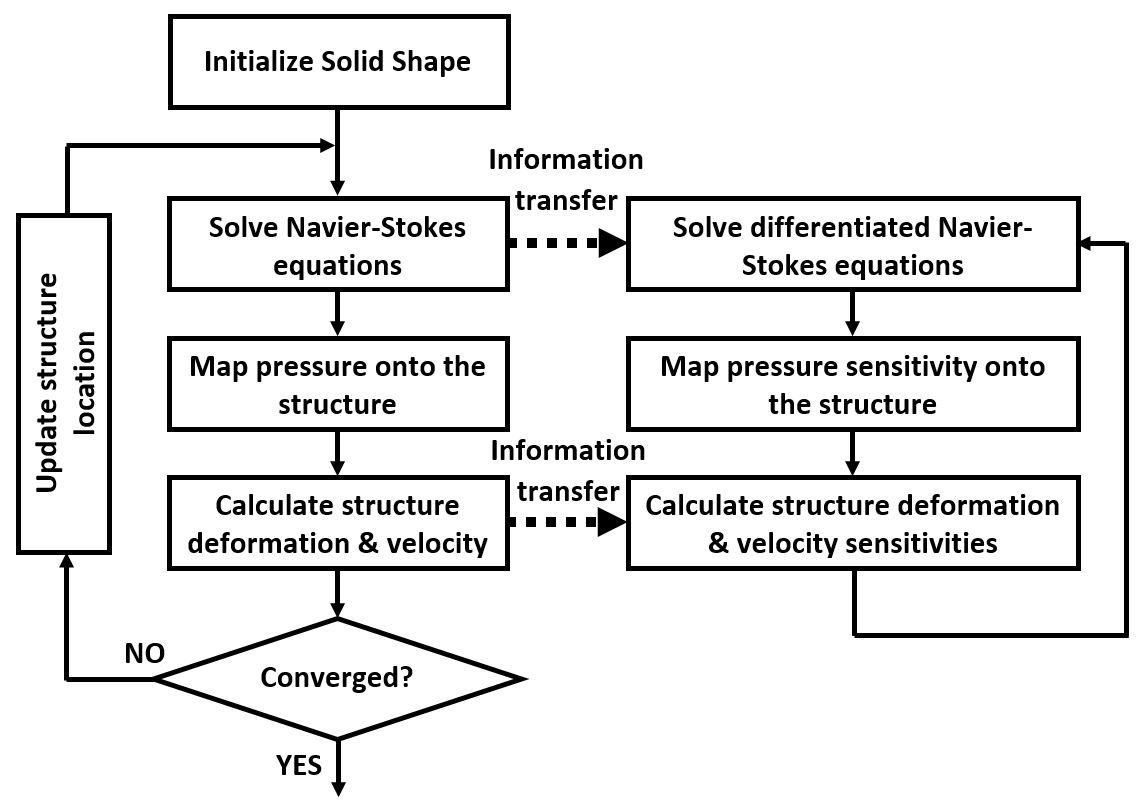
\includegraphics[width=14.00cm]{Chapter_5/figure/couple_SA_flowchart.jpg}
    \caption{Coupled multidisciplinary sensitivity analysis flowchart.}
    \label{fig:C5_SAflowchart}
\end{figure}
%